Im folgenden Abschnitt sind die während des Versuchs aufgenommenen 
und die daraus berechneten Daten tabellarisch und grafisch dargestellt.
An entsprechender Stelle sind Erklärungen zu den vorgenommenen Berechnungen 
und Ergebnissen gegeben. Die für die Fehlerrechnung verwendeten Gleichungen
befinden sich in \cref{sec:Fehlerrechnung} und werden mit römischen Ziffern
referenziert.

\subsection{Überprüfung der bekannten Brennweite einer Linse}

	Die Messwerte, die für die Berechnung und Überprüfung der Brennweite $f=\SI{10}{\centi\meter}$ aufgenommen wurden 
	befinden sich in \cref{tab:Auswertung_Messwerte_I}.
	Aus diesen wurden die Bildweiten nach $b = \envert{x_{B} - x_{L}}$ und die Gegenstandsweitenh 
	nach  $g = \envert{x_{G} - x_{L}}$ berechnet. Für die Position des Gegenstands wurde dazu $x_{G} = \SI{129.0(1)}{\cm}$ gemessen.
	
	
	\begin{table}[!h]
	\centering
	\begin{tabular}{|c|c|c|c|}
		\hline
		Pos. Bild & Pos. Linse & Gegenstandsweite & Bildweite\\
		$x_{B}$ [\si{\centi\meter}] & $x_{L}$ [\si{\centi\meter}] & $g$ [\si{\centi\meter}] & $b$ [\si{\centi\meter}]\\
\hline\hline
		\num{89.6(1)} & \num{109.0(1)} & \num{20.0(1)} & \num{19.4(1)}\\
		\num{87.8(1)} & \num{104.0(1)} & \num{25.0(1)} & \num{16.2(1)}\\
		\num{84.4(1)} & \num{99.0(1)} & \num{30.0(1)} & \num{14.6(1)}\\
		\num{80.4(1)} & \num{94.0(1)} & \num{35.0(1)} & \num{13.6(1)}\\
		\num{76.0(1)} & \num{89.0(1)} & \num{40.0(1)} & \num{13.0(1)}\\
		\num{71.5(1)} & \num{84.0(1)} & \num{45.0(1)} & \num{12.5(1)}\\
		\num{66.9(1)} & \num{79.0(1)} & \num{50.0(1)} & \num{12.1(1)}\\
		\num{62.1(1)} & \num{74.0(1)} & \num{55.0(1)} & \num{11.9(1)}\\
		\num{57.2(1)} & \num{69.0(1)} & \num{60.0(1)} & \num{11.8(1)}\\
		\num{52.4(1)} & \num{64.0(1)} & \num{65.0(1)} & \num{11.6(1)}\\
		\hline
	\end{tabular}
	\caption{Gemessene Positionen des Bildes und der Linse und die daraus bestimmten 
		Bild- und Gegenstandsweiten für die Messreihe mit der bekannten Linse. Als Fehler wurde die kleinste Skaleneinteilung des
		verwendeten Millimetermaßes angenommen.  \label{tab:Auswertung_Messwerte_I}}
\end{table}
  			
	
	In \cref{fig:Auswertung_BekannteLinse} sind die Geraden durch den Wert von $b$ auf der y-Achse und den Wert von $g$
	auf der x-Achse eingezeichnet. Der Schnittpunkt dieser Geraden liegt im Punkt $(f|f)$, wobei $f$
	die Brennweite der Linse ist. 
	  
	\begin{figure}[!h]
		\centering
		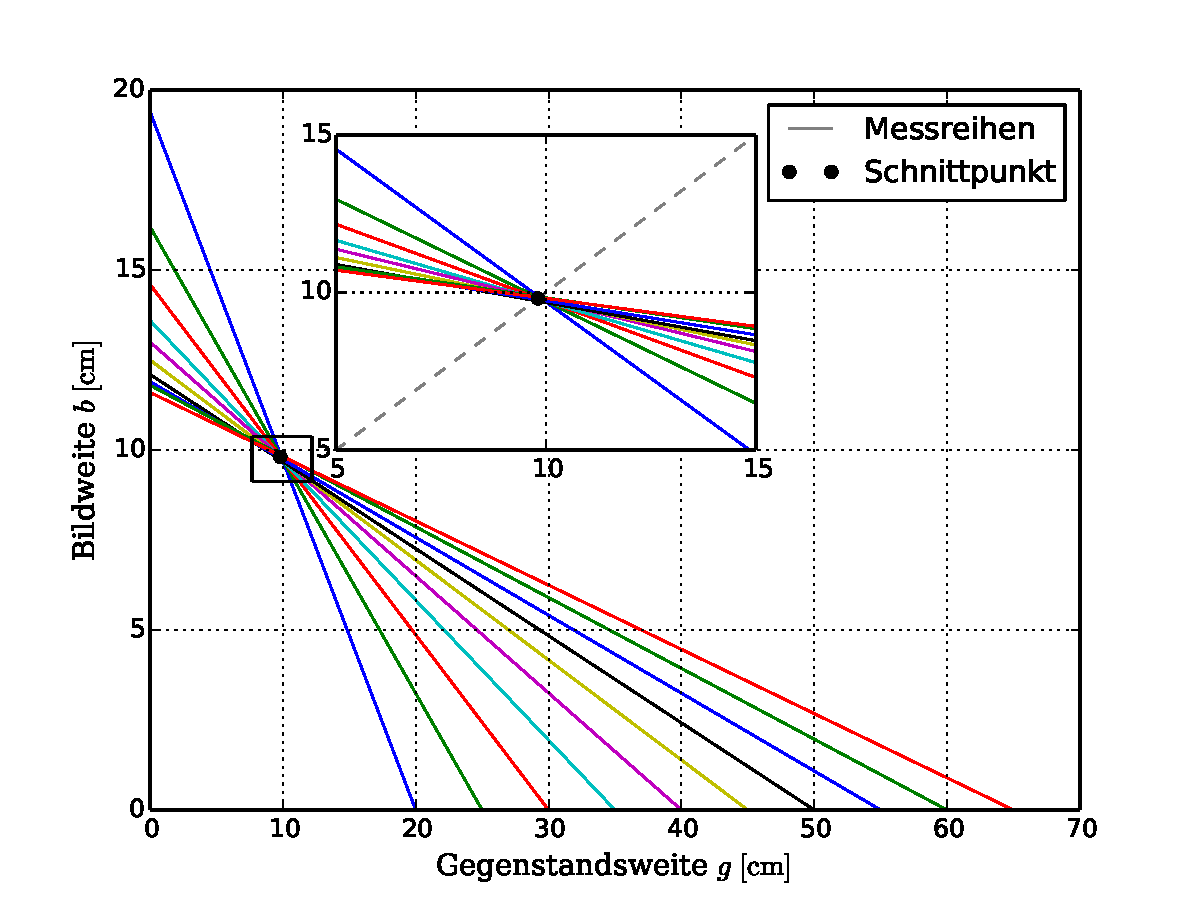
\includegraphics[scale=.7]{Grafiken/Messwerte_Bekannt.pdf}
		\caption{Graphische Auswertung der Messwerte der Messreihe mit bekannter Linse \label{fig:Auswertung_BekannteLinse}}
	\end{figure}  
	 
	 Der Schnittpunkt, tatsächlich schneiden sich die Geraden nicht in einem Punkt, der Wert
	 des eingezeichneten Schnittpunktes ist der Mittelwert der Brennweiten, die mit der Linsengleichung
	 \cref{eq:Theorie_Linsengln} berechnet
	 wurden, der Geraden liegt bei $(9.82|9.82)$ erhält man für die Brennweite der Linse
	 \begin{empheq}{equation}
		\label{val:Auswertung_Bekannt}
		\mean{f} = \SI{9.81(2)}{\centi\meter}.
	 \end{empheq}
	 Der Fehler der Brennweite wurde dabei durch Gaußsche Fehlerfortpflanzung bestimmt, da dieser Fehler größer als
	 die Abweichung vom Mittelwert ist.	 
	 
	 Zur Überprüfung der Abbildungsgesetzes \cref{eq:Theorie_Abbildungsgesetz} wurden in 
	 Messung 2 mit $g_{2} = \SI{25.0(1)}{\cm}$ und $b_{2} = \SI{16.2(1)}{\cm}$ sowie
	 bei Messung 5 mit $g_{5} = \SI{40.0(1)}{\cm}$ und $b_{5} = \SI{13.0(1)}{\cm}$
	 die Bildgröße $B_{2} = \SI{2.0(1)}{\cm}$ bzw. $B_{5} = \SI{1.0(1)}{\cm}$ und 
	 die Gegenstandsgröße $G = \SI{3.0(1)}{\centi\meter}$ gemessen.
	 Die beiden Seiten des Abbildungsgesetz ergeben damit jeweils:
	 \begin{empheq}{alignat* = 2}
%	 	&\text{Messung 2:} \qquad &\text{Messung 5:}	\\
	 	&\dfrac{g_{2}}{b_{2}} = \SI{1.54(2)}{\cm} \qquad	&\dfrac{g_{5}}{b_{5}} = \SI{3.08(4)}{\cm}\\  
	 	&\dfrac{G}{B_{2}} = \SI{1.50(9)}{\cm}	\qquad     &\dfrac{G}{B_{5}} = \SI{3.0(3)}{\cm}
	 \end{empheq}
	 
	 
	  
\subsection{Bestimmung der unbekannten Brennweite einer Linse}
	
	Die zur Bestimmung der Brennweite der unbekannten Linse aufgenommenen Daten sind in 
	\cref{tab:Auswertung_Messwerte_II} zu finden.
	
	\begin{table}[!h]
	\centering
	\begin{tabular}{|c|c|c|c|c||c|}
		\hline
		Messreihe & 1 & 2 & 3 & 4 & Verschiebung\\
		Nr. &$$ & $$ & $$ & $$ & $D$ [\si{\centi\meter}]\\
\hline
\multirow{7}{1.75cm}{Ablenk-\\ strom\\$\quad\!I_{d}$\ [\si{\ampere}]}		&\num{0.00(1)} & \num{0.00(1)} & \num{0.00(1)} & \num{0.00(1)} & \num{0.0(1)}\\
		&\num{0.32(1)} & \num{0.36(1)} & \num{0.38(1)} & \num{0.38(1)} & \num{0.6(1)}\\
		&\num{0.68(1)} & \num{0.74(1)} & \num{0.82(1)} & \num{0.84(1)} & \num{1.3(1)}\\
		&\num{1.00(1)} & \num{1.10(1)} & \num{1.20(1)} & \num{1.15(1)} & \num{1.9(1)}\\
		&\num{1.30(1)} & \num{1.45(1)} & \num{1.60(1)} & \num{1.60(1)} & \num{2.5(1)}\\
		&\num{1.65(1)} & \num{1.80(1)} & \num{1.95(1)} & \num{2.00(1)} & \num{3.2(1)}\\
		&\num{2.00(1)} & \num{2.20(1)} & - & - & \num{3.8(1)}\\
		&\num{2.25(1)} & - & - & - & \num{4.4(1)}\\ \hline
\multirow{3}{1.75cm}{Beschl.\\Spannung\\$\quad\!U_{b}$\ [\si{\volt}]}	& & & & & \\
				 							   & \num{250(5)}   &   \num{300(5)}  & \num{350(5)}  & \num{400(5)} &  
				 							   \\ 
				 							   &&&&&\\\hline
		
		
		\hline
	\end{tabular}
	\caption{Messdaten zur Bestimmung des Zusammenhangs zwischen $I_d$ und $D$ \label{tab:Auswertung_Messdaten_II}}
\end{table}
 
	
	In \cref{fig:Auswertung_UnbekannteLinse} sind die Werte aus \cref{tab:Auswertung_Messwerte_II} und der gemittelte Schnittpunkt
	$(7.52|7.52)$ aufgetragen.
	
	\begin{figure}[!h]
		\centering
		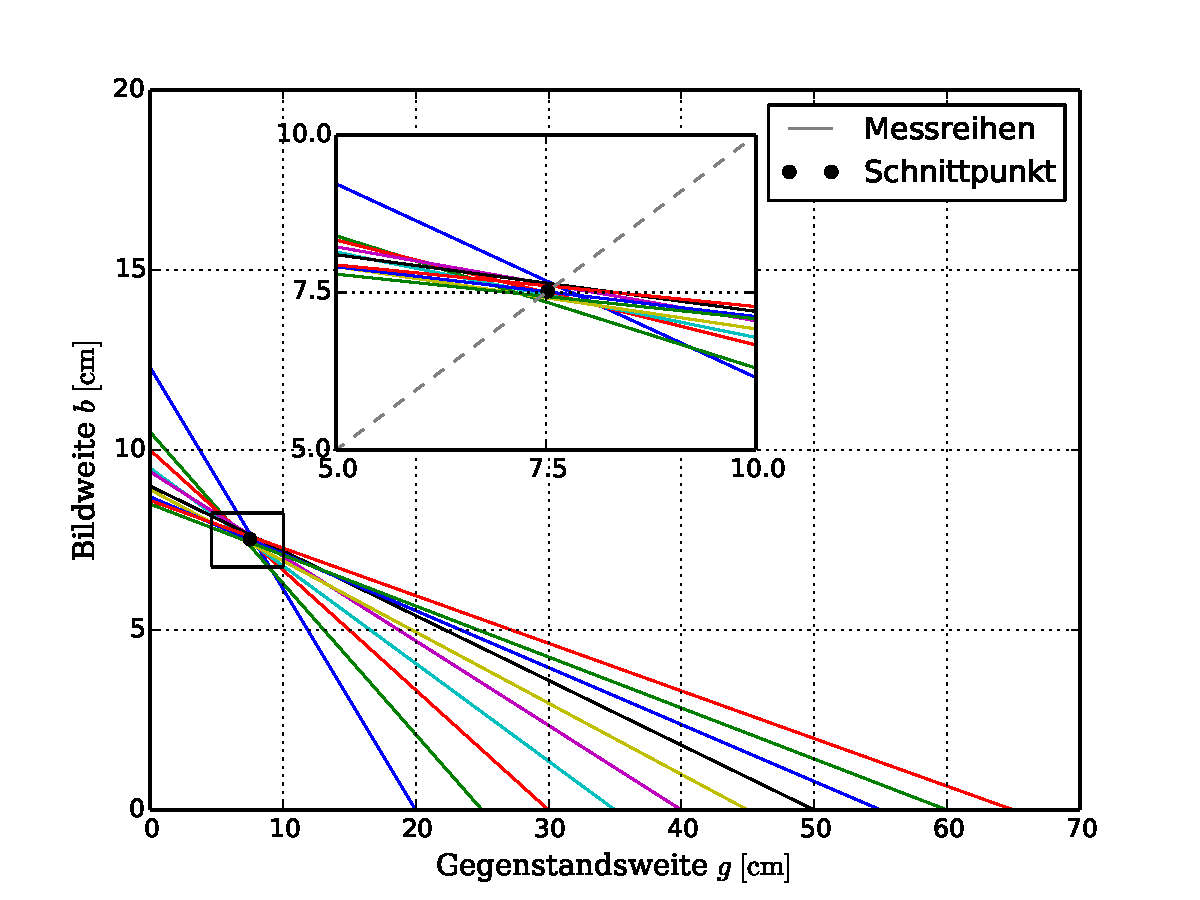
\includegraphics[scale=.7]{Grafiken/Messwerte_Unbekannt.pdf}
		\caption{Graphische Auswertung der Messwerte der Messreihe mit unbekannter Linse \label{fig:Auswertung_UnbekannteLinse}}
	\end{figure}  
	
	
	Daraus erhält man die unbekannte Brennweite der Linse mit 
	 \begin{empheq}{equation}
			\label{val:Auswertung_Unbekannt}
			\mean{f} = \SI{7.52(3)}{\centi\meter}.
	 \end{empheq}
	Auch der hier bestimmte Fehler der Brennweite wurde mit Hilfe der gaußschen Fehlerfortpflanzung bestimmt,
	da dieser die Abweichung vom Mittelwert übersteigt. 

\subsection{Überprüfung der bekannten Brennweite einer Linse nach Bessel}

	\subsubsection{Unter Verwendung von weißem Licht}
	
		Die während des Versuchs gemessenen Position des Bildschirms $x_{B}$ und
		die beiden Positionen der Linse $x_{L,1}$ und $x_{L,2}$ in \cref{tab:Auswertung_Messwerte_III} eingetragen. 
		Aus diesen wurden, mit der festen Position des Gegenstands $x_{G} = \SI{129.0(1)}{\centi\meter}$,
		Linsenabstand $d = \envert{x_{L,1} - x_{L,2}}$ und Gesamtabstand $e = \envert{x_{G}- x_{B}}$ 
		berechnet. Mit \cref{eq:Theorie_Bessel} lässt sich aus diesen die Brennweite $f$ der Linse bestimmen.
		
		\begin{table}[!h]
	\centering
	\begin{tabular}{|c|c|}
		\hline
		Versuch Nr. & Anzahl Pulse\\
\hline\hline
		\num{1} & \num{569}\\
		\num{2} & \num{616}\\
		\num{3} & \num{590}\\
		\num{4} & \num{566}\\
		\num{5} & \num{599}\\
		\num{6} & \num{627}\\
		\num{7} & \num{612}\\
		\num{8} & \num{604}\\
		\num{9} & \num{596}\\
		\num{10} & \num{618}\\
		\num{11} & \num{617}\\
		\num{12} & \num{621}\\
		\num{13} & \num{634}\\
		\num{14} & \num{603}\\
		\num{15} & \num{588}\\
		\num{16} & \num{669}\\
		\num{17} & \num{633}\\
		\num{18} & \num{630}\\
		\num{19} & \num{618}\\
		\num{20} & \num{590}\\
		\num{21} & \num{593}\\
		\num{22} & \num{595}\\
		\num{23} & \num{575}\\
		\num{24} & \num{600}\\
		\num{25} & \num{682}\\
		\num{26} & \num{636}\\
		\num{27} & \num{639}\\
		\num{28} & \num{670}\\
		\num{29} & \num{601}\\
		\num{30} & \num{628}\\
		\num{31} & \num{652}\\
		\num{32} & \num{599}\\
		\num{33} & \num{663}\\
		\num{34} & \num{617}\\
		\num{35} & \num{1223}\\
		\num{36} & \num{1308}\\
		\num{37} & \num{841}\\
		\num{38} & \num{647}\\
		\num{39} & \num{598}\\
		\num{40} & \num{633}\\
		\num{41} & \num{645}\\
		\num{42} & \num{593}\\
		\num{43} & \num{573}\\
		\num{44} & \num{603}\\
		\num{45} & \num{561}\\
		\num{46} & \num{645}\\
		\num{47} & \num{611}\\
		\num{48} & \num{575}\\
		\num{49} & \num{590}\\
		\num{50} & \num{591}\\
		\num{51} & \num{692}\\
		\num{52} & \num{601}\\
		\num{53} & \num{655}\\
		\num{54} & \num{776}\\
		\num{55} & \num{783}\\
		\num{56} & \num{997}\\
		\num{57} & \num{838}\\
		\num{58} & \num{683}\\
		\num{59} & \num{681}\\
		\num{60} & \num{815}\\
		\num{61} & \num{628}\\
		\num{62} & \num{670}\\
		\num{63} & \num{652}\\
		\num{64} & \num{623}\\
		\num{65} & \num{620}\\
		\num{66} & \num{719}\\
		\num{67} & \num{858}\\
		\num{68} & \num{597}\\
		\num{69} & \num{658}\\
		\num{70} & \num{638}\\
		\num{71} & \num{649}\\
		\num{72} & \num{688}\\
		\num{73} & \num{707}\\
		\num{74} & \num{896}\\
		\num{75} & \num{844}\\
		\num{76} & \num{593}\\
		\num{77} & \num{746}\\
		\num{78} & \num{1089}\\
		\num{79} & \num{674}\\
		\num{80} & \num{754}\\
		\num{81} & \num{750}\\
		\num{82} & \num{834}\\
		\num{83} & \num{795}\\
		\num{84} & \num{703}\\
		\num{85} & \num{858}\\
		\num{86} & \num{702}\\
		\num{87} & \num{636}\\
		\num{88} & \num{599}\\
		\num{89} & \num{1206}\\
		\num{90} & \num{664}\\
		\num{91} & \num{609}\\
		\num{92} & \num{660}\\
		\num{93} & \num{662}\\
		\num{94} & \num{663}\\
		\num{95} & \num{689}\\
		\num{96} & \num{644}\\
		\num{97} & \num{648}\\
		\num{98} & \num{604}\\
		\num{99} & \num{613}\\
		\num{100} & \num{581}\\
		\hline
	\end{tabular}
	\caption{Anzahl der gemessenen Impulse \label{tab:Messwerte_III}}
\end{table}

		
		Daraus ergibt sich der Mittelwert für die Brennweite der Linse,
		mit dem durch gaußschen Fortpflanzung bestimmten Fehler,  zu
		\begin{empheq}{equation}
			\label{val:Auswertung_BesselWeis}
			\mean{f_{weiss}} = \SI{9.93(4)}{\centi\meter}.
		\end{empheq}
		
	\subsubsection{Unter Verwendung von rotem Licht}	
		
		In \cref{tab:Auswertung_Messwerte_III_r} sind die Messwerte der mit rotem
		Licht durchgeführten Methode von Bessel sowie die aus diesen berechneten
		Größen zu finden.
		
		\begin{table}[!h]
	\centering
	\begin{tabular}{|c|c|c|c|c|c|}
		\hline
		Pos. Bild & Pos. Linse 1 & Pos. Linse 2 & Linsenabstand & Gesamtabstand & Brennweite\\
		$x_{B}$ [\si{\centi\meter}] & $x_{L,1}$ [\si{\centi\meter}] & $x_{L,2}$ [\si{\centi\meter}] & $d$ [\si{\centi\meter}] & $e$ [\si{\centi\meter}] & $f_{rot}$ [\si{\centi\meter}]\\
\hline\hline
		\num{88.2(1)} & \num{105.2(1)} & \num{111.4(1)} & \num{6.2(1)} & \num{40.8(1)} & \num{9.96(4)}\\
		\num{85.0(1)} & \num{100.0(1)} & \num{113.5(1)} & \num{13.5(1)} & \num{44.0(1)} & \num{9.96(4)}\\
		\num{80.0(1)} & \num{93.7(1)} & \num{114.7(1)} & \num{21.0(1)} & \num{49.0(1)} & \num{10.00(5)}\\
		\num{75.0(1)} & \num{88.0(1)} & \num{115.5(1)} & \num{27.5(1)} & \num{54.0(1)} & \num{10.00(6)}\\
		\num{70.0(1)} & \num{82.5(1)} & \num{115.9(1)} & \num{33.4(1)} & \num{59.0(1)} & \num{10.02(6)}\\
		\hline
	\end{tabular}
	\caption{Messwerte der Position des Bildes und der beiden Linsen Positionen    und zur Berechnung der Brennweite nach Bessel bestimmte Abstände, für die Durchführung mit rotem Licht. \label{tab:Auswertung_Messwerte_III_r}}
\end{table}

		
		 Der Mittelwert der Brennweite von rotem Licht ergibt sich aus diesen Daten zu
		\begin{empheq}{equation}
			\label{val:Auswertung_BesselRot}
			\mean{f_{rot}} = \SI{9.99(4)}{\centi\meter}.
		\end{empheq}		 
		
	
	\subsubsection{Unter Verwendung von blauem Licht}	
		
		Die Messung nach der Methode von Bessel mit blauem Licht ergab die 
		in \cref{tab:Auswertung_Messwerte_III_b}  dargestellten Messwerte und Ergebnisse.	
		
		\begin{table}[!h]
	\centering
	\begin{tabular}{|c|c|c|c|c|c|}
		\hline
		Pos. Bild & Pos. Linse 1 & Pos. Linse 2 & Linsenabstand & Gesamtabstand & Brennweite\\
		$x_{B}$ [\si{\centi\meter}] & $x_{L,1}$ [\si{\centi\meter}] & $x_{L,2}$ [\si{\centi\meter}] & $d$ [\si{\centi\meter}] & $e$ [\si{\centi\meter}] & $f_{blau}$ [\si{\centi\meter}]\\
\hline\hline
		\num{88.2(1)} & \num{103.8(1)} & \num{112.5(1)} & \num{8.7(1)} & \num{40.8(1)} & \num{9.74(4)}\\
		\num{85.0(1)} & \num{99.5(1)} & \num{113.9(1)} & \num{14.4(1)} & \num{44.0(1)} & \num{9.82(5)}\\
		\num{80.0(1)} & \num{93.7(1)} & \num{115.0(1)} & \num{21.3(1)} & \num{49.0(1)} & \num{9.94(5)}\\
		\num{75.0(1)} & \num{88.0(1)} & \num{115.7(1)} & \num{27.7(1)} & \num{54.0(1)} & \num{9.95(6)}\\
		\num{70.0(1)} & \num{82.5(1)} & \num{116.0(1)} & \num{33.5(1)} & \num{59.0(1)} & \num{9.99(6)}\\
		\hline
	\end{tabular}
	\caption{Messwerte und Ergebnisse nach Bessel mit blauem Licht \label{tab:Auswertung_Messwerte_III_b}}
\end{table}
		
		
		Für blaues Licht ergibt sich der Mittelwert der Brennweite zu
		\begin{empheq}{equation}
			\label{val:Auswertung_BesselBlau}
			\mean{f_{blau}} = \SI{9.89(4)}{\centi\meter}.
		\end{empheq}		
		
		

\subsection{Bestimmung der unbekannten Brennweite eines Linsensystems nach Abbe}
	
	Die für die Bestimmung der Brennweite des Linsensystems aus konkaver und konvexer Linse
	aufgenommenen Messwerte für Bild- und Referenzpunktposition $x_{B}$ und $x_{A}$ sowie 
	der Bildgröße $B$ sind in \cref{tab:Auswertung_Messwerte_VI} zu finden. Für die Berechnung der nötigen Werte
	wurden noch die Gegenstandsgröße $G = \SI{3.0(1)}{\centi\meter}$ und 
	-position $x_{G} = \SI{129.0(1)}{\centi\meter}$ verwandt.   
	
	\begin{table}[!h]
	\centering
	\begin{adjustbox}{width=1\textwidth, center}
	\begin{tabular}{|c|c|c|c|c|c|}
		\hline
		Pos. Bild & Pos. Referenzpunkt & Bildgröße & Gegenstandsweite & Bildweite & Abbildungsmaßstab\\
		$x_{B}$ [\si{\centi\meter}] & $x_{A}$ [\si{\centi\meter}] & $B$ [\si{\centi\meter}] & $g'$ [\si{\centi\meter}] & $b'$ [\si{\centi\meter}] & $V$\\
\hline\hline
		\num{4.0(1)} & \num{105.7(1)} & \num{7.4(1)} & \num{23.3(1)} & \num{101.7(1)} & \num{2.47(9)}\\
		\num{10.0(1)} & \num{104.1(1)} & \num{6.7(1)} & \num{24.9(1)} & \num{94.1(1)} & \num{2.23(8)}\\
		\num{12.0(1)} & \num{103.3(1)} & \num{6.3(1)} & \num{25.7(1)} & \num{91.3(1)} & \num{2.10(8)}\\
		\num{15.0(1)} & \num{102.4(1)} & \num{5.7(1)} & \num{26.6(1)} & \num{87.4(1)} & \num{1.90(7)}\\
		\num{17.0(1)} & \num{98.5(1)} & \num{4.8(1)} & \num{30.5(1)} & \num{81.5(1)} & \num{1.60(6)}\\
		\num{20.0(1)} & \num{98.2(1)} & \num{4.7(1)} & \num{30.8(1)} & \num{78.2(1)} & \num{1.57(6)}\\
		\num{22.0(1)} & \num{97.2(1)} & \num{4.2(1)} & \num{31.8(1)} & \num{75.2(1)} & \num{1.40(6)}\\
		\num{25.0(1)} & \num{96.1(1)} & \num{3.7(1)} & \num{32.9(1)} & \num{71.1(1)} & \num{1.23(5)}\\
		\num{27.0(1)} & \num{94.2(1)} & \num{3.5(1)} & \num{34.8(1)} & \num{67.2(1)} & \num{1.17(5)}\\
		\num{30.0(1)} & \num{93.2(1)} & \num{3.4(1)} & \num{35.8(1)} & \num{63.2(1)} & \num{1.13(5)}\\
		\hline
	\end{tabular}
	\end{adjustbox}
	\caption{Messwerte und Ergebnisse nach der Methode von Abbe \label{tab:Auswertung_Messwerte_VI}}
\end{table}

	
	Die Werte für $g'$ bzw. $b'$ aus \cref{tab:Auswertung_Messwerte_VI} sind in
	\cref{fig:Auswertung_AbbeG} bzw. \cref{fig:Auswertung_AbbeB}  gegen $(1 + V^{-1})$ bzw. $(1 + V)$ aufgetragen.
	Durch lineare Regression, mittels der Pythonbibliothek \emph{SciPy} \cite{SciPy}, beider Messwertepaare 
	mit dem Ansatz
	\begin{empheq}{equation}
		m(x) = f\cdot x + b
	\end{empheq}
	erhält man die Geradenparameter für $g'$ \cref{eq:Theorie_g'}
	\begin{subequations}
	 	\begin{empheq}{align}
	 		f_{g} &= \SI{25(1)}{\centi\meter}\\
	 		b &= h = \SI{-11(2)}{\centi\meter}
	 	\end{empheq}
	\end{subequations}
	und für $b'$ \cref{eq:Theorie_b'} 
	\begin{subequations}
	 	\begin{empheq}{align}
	 		f_{b} &= \SI{26(1)}{\centi\meter}\\
	 		b &= h' = \SI{11(4)}{\centi\meter}.
	 	\end{empheq}
	\end{subequations}

	\begin{figure}[!h]
		\centering
		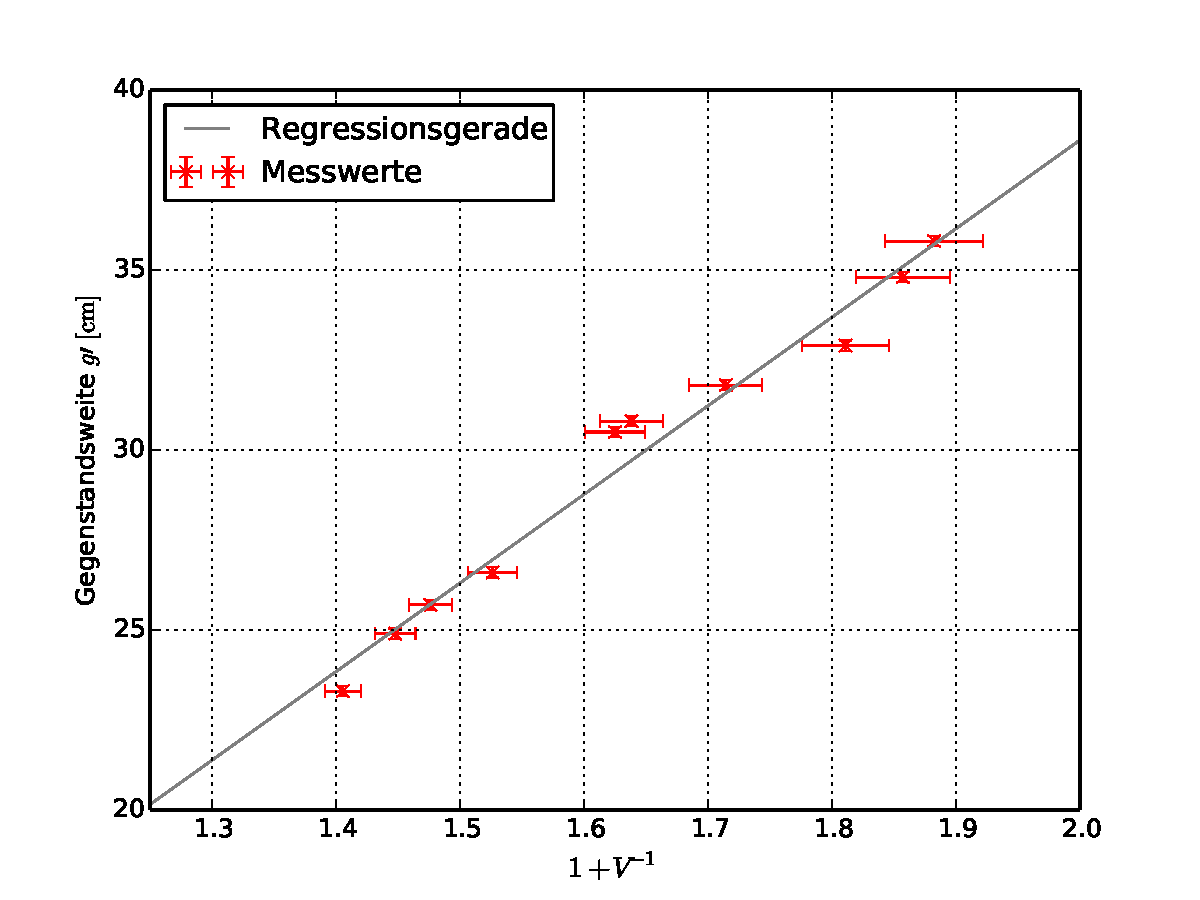
\includegraphics[scale=.7]{Grafiken/Messwerte_Abbe2.pdf}
		\caption{Regression der Messwerte der gestrichenen Gegenstandsweiten\label{fig:Auswertung_AbbeG}}
	\end{figure}
	
	\begin{figure}[!h]
		\centering
		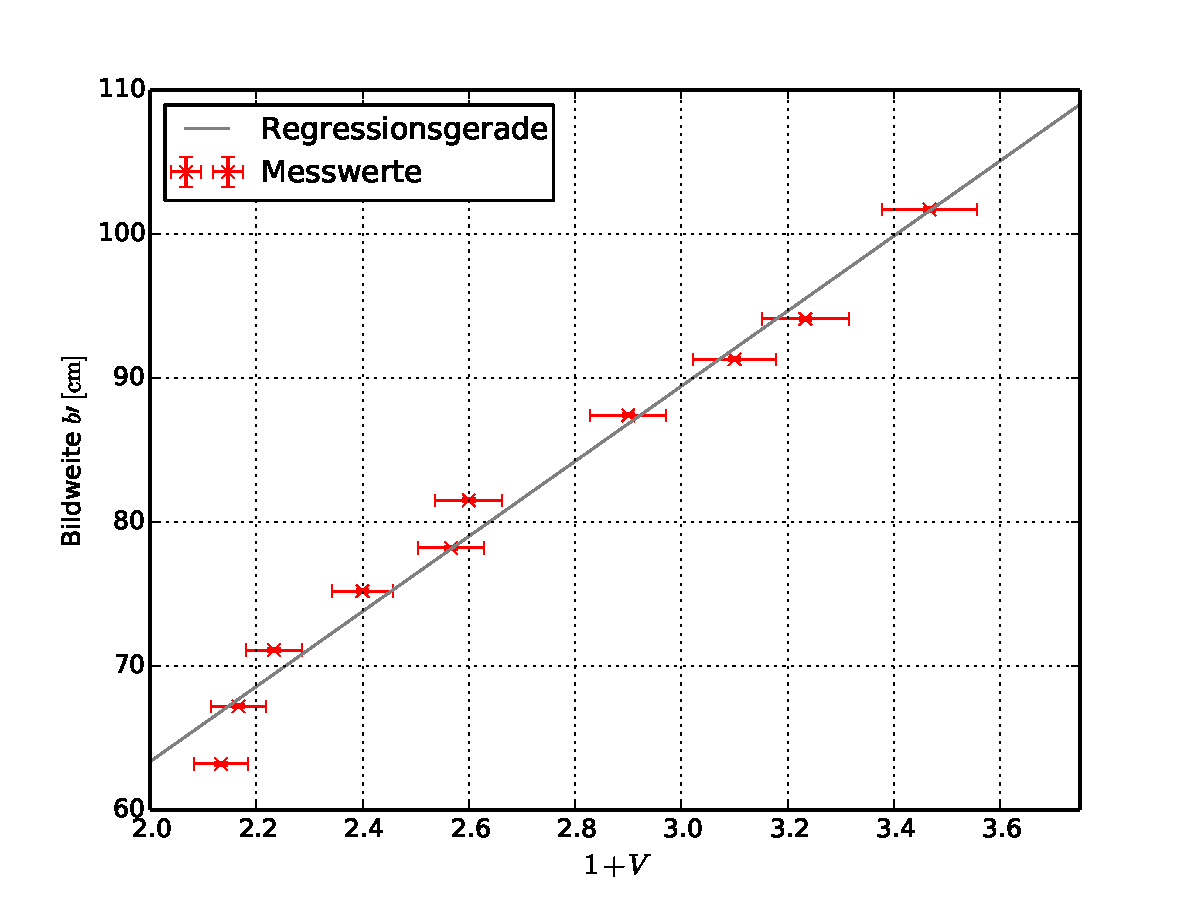
\includegraphics[scale=.7]{Grafiken/Messwerte_Abbe1.pdf}
		\caption{Regression der Messwerte der gestrichenen Bildweite\label{fig:Auswertung_AbbeB}}
	\end{figure}
	
	
	
	
	Da die Steigungen dieser Geraden jeweils die Brennweite des Linsensystems darstellt ergibt sich
	diese im Mittel zu
 	\begin{empheq}{equation}
 		\label{val:Auswertung_Abbe}
 		\mean{f} = \SI{25.5(7)}{\centi\meter}.
 	\end{empheq}
 	
 	Die eine der beiden Hauptebenen des Systems liegt ca. \SI{11}{\centi\meter} vor,
 	und die zweite Hauptebene ca. \SI{11(2)}{\centi\meter} hinter dem gewählten 
 	Referenzpunkt (der Position der konkaven Linse).  
 	